%!TeX root=../princesstop.tex
\chapter{Ermengarde}

\begin{figure}[t!]
\centering
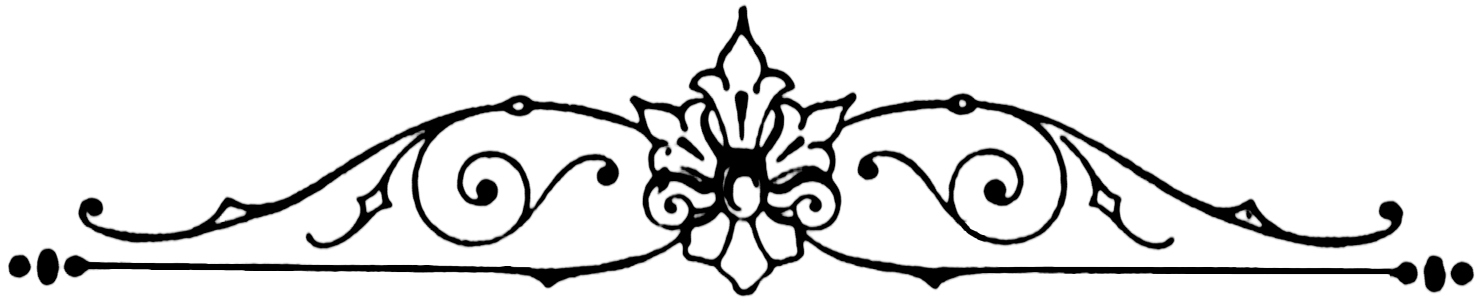
\includegraphics[width=\linewidth]{filigree}
\end{figure}

\lettrine[lines=5]{O}{n} that first morning, when Sara sat at Miss Minchin's side, aware that the whole schoolroom was devoting itself to observing her, she had noticed very soon one little girl, about her own age, who looked at her very hard with a pair of light, rather dull, blue eyes. She was a fat child who did not look as if she were in the least clever, but she had a good-naturedly pouting mouth. Her flaxen hair was braided in a tight pigtail, tied with a ribbon, and she had pulled this pigtail around her neck, and was biting the end of the ribbon, resting her elbows on the desk, as she stared wonderingly at the new pupil. When Monsieur Dufarge began to speak to Sara, she looked a little frightened; and when Sara stepped forward and, looking at him with the innocent, appealing eyes, answered him, without any warning, in French, the fat little girl gave a startled jump, and grew quite red in her awed amazement. Having wept hopeless tears for weeks in her efforts to remember that <la mère> meant <the mother,> and <le père,> <the father,>—when one spoke sensible English—it was almost too much for her suddenly to find herself listening to a child her own age who seemed not only quite familiar with these words, but apparently knew any number of others, and could mix them up with verbs as if they were mere trifles.

She stared so hard and bit the ribbon on her pigtail so fast that she attracted the attention of Miss Minchin, who, feeling extremely cross at the moment, immediately pounced upon her.

<Miss St John!> she exclaimed severely. <What do you mean by such conduct? Remove your elbows! Take your ribbon out of your mouth! Sit up at once!>

Upon which Miss St John gave another jump, and when Lavinia and Jessie tittered she became redder than ever—so red, indeed, that she almost looked as if tears were coming into her poor, dull, childish eyes; and Sara saw her and was so sorry for her that she began rather to like her and want to be her friend. It was a way of hers always to want to spring into any fray in which someone was made uncomfortable or unhappy.

<If Sara had been a boy and lived a few centuries ago,> her father used to say, <she would have gone about the country with her sword drawn, rescuing and defending everyone in distress. She always wants to fight when she sees people in trouble.>

So she took rather a fancy to fat, slow, little Miss St John, and kept glancing toward her through the morning. She saw that lessons were no easy matter to her, and that there was no danger of her ever being spoiled by being treated as a show pupil. Her French lesson was a pathetic thing. Her pronunciation made even Monsieur Dufarge smile in spite of himself, and Lavinia and Jessie and the more fortunate girls either giggled or looked at her in wondering disdain. But Sara did not laugh. She tried to look as if she did not hear when Miss St John called <le bon pain,> <lee bong pang.> She had a fine, hot little temper of her own, and it made her feel rather savage when she heard the titters and saw the poor, stupid, distressed child's face.

<It isn't funny, really,> she said between her teeth, as she bent over her book. <They ought not to laugh.>

When lessons were over and the pupils gathered together in groups to talk, Sara looked for Miss St John, and finding her bundled rather disconsolately in a window-seat, she walked over to her and spoke. She only said the kind of thing little girls always say to each other by way of beginning an acquaintance, but there was something friendly about Sara, and people always felt it.

<What is your name?> she said.

To explain Miss St John's amazement one must recall that a new pupil is, for a short time, a somewhat uncertain thing; and of this new pupil the entire school had talked the night before until it fell asleep quite exhausted by excitement and contradictory stories. A new pupil with a carriage and a pony and a maid, and a voyage from India to discuss, was not an ordinary acquaintance.

<My name's Ermengarde St John,> she answered.

<Mine is Sara Crewe,> said Sara. <Yours is very pretty. It sounds like a story book.>

<Do you like it?> fluttered Ermengarde. <I—I like yours.>

Miss St John's chief trouble in life was that she had a clever father. Sometimes this seemed to her a dreadful calamity. If you have a father who knows everything, who speaks seven or eight languages, and has thousands of volumes which he has apparently learned by heart, he frequently expects you to be familiar with the contents of your lesson books at least; and it is not improbable that he will feel you ought to be able to remember a few incidents of history and to write a French exercise. Ermengarde was a severe trial to Mr St John. He could not understand how a child of his could be a notably and unmistakably dull creature who never shone in anything.

<Good heavens!> he had said more than once, as he stared at her, <there are times when I think she is as stupid as her Aunt Eliza!>

If her Aunt Eliza had been slow to learn and quick to forget a thing entirely when she had learned it, Ermengarde was strikingly like her. She was the monumental dunce of the school, and it could not be denied.

<She must be \textsc{made} to learn,> her father said to Miss Minchin.

Consequently Ermengarde spent the greater part of her life in disgrace or in tears. She learned things and forgot them; or, if she remembered them, she did not understand them. So it was natural that, having made Sara's acquaintance, she should sit and stare at her with profound admiration.

<You can speak French, can't you?> she said respectfully.

Sara got on to the window-seat, which was a big, deep one, and, tucking up her feet, sat with her hands clasped round her knees.

<I can speak it because I have heard it all my life,> she answered. <You could speak it if you had always heard it.>

<Oh, no, I couldn't,> said Ermengarde. <I \textsc{never} could speak it!>

<Why?> inquired Sara, curiously.

Ermengarde shook her head so that the pigtail wobbled.

<You heard me just now,> she said. <I'm always like that. I can't \textsc{say} the words. They're so queer.>

She paused a moment, and then added with a touch of awe in her voice, <You are \textsc{clever}, aren't you?>

Sara looked out of the window into the dingy square, where the sparrows were hopping and twittering on the wet, iron railings and the sooty branches of the trees. She reflected a few moments. She had heard it said very often that she was <clever,> and she wondered if she was—and \textsc{if} she was, how it had happened.

<I don't know,> she said. <I can't tell.> Then, seeing a mournful look on the round, chubby face, she gave a little laugh and changed the subject.

<Would you like to see Emily?> she inquired.

<Who is Emily?> Ermengarde asked, just as Miss Minchin had done.

<Come up to my room and see,> said Sara, holding out her hand.

They jumped down from the window-seat together, and went upstairs.

<Is it true,> Ermengarde whispered, as they went through the hall—<is it true that you have a playroom all to yourself?>

<Yes,> Sara answered. <Papa asked Miss Minchin to let me have one, because—well, it was because when I play I make up stories and tell them to myself, and I don't like people to hear me. It spoils it if I think people listen.>

They had reached the passage leading to Sara's room by this time, and Ermengarde stopped short, staring, and quite losing her breath.

<You \textsc{make} up stories!> she gasped. <Can you do that—as well as speak French? \textsc{Can} you?>

Sara looked at her in simple surprise.

<Why, anyone can make up things,> she said. <Have you never tried?>

She put her hand warningly on Ermengarde's.

<Let us go very quietly to the door,> she whispered, <and then I will open it quite suddenly; perhaps we may catch her.>

She was half laughing, but there was a touch of mysterious hope in her eyes which fascinated Ermengarde, though she had not the remotest idea what it meant, or whom it was she wanted to <catch,> or why she wanted to catch her. Whatsoever she meant, Ermengarde was sure it was something delightfully exciting. So, quite thrilled with expectation, she followed her on tiptoe along the passage. They made not the least noise until they reached the door. Then Sara suddenly turned the handle, and threw it wide open. Its opening revealed the room quite neat and quiet, a fire gently burning in the grate, and a wonderful doll sitting in a chair by it, apparently reading a book.

<Oh, she got back to her seat before we could see her!> Sara explained. <Of course they always do. They are as quick as lightning.>

Ermengarde looked from her to the doll and back again.

<Can she—walk?> she asked breathlessly.

<Yes,> answered Sara. <At least I believe she can. At least I \textsc{pretend} I believe she can. And that makes it seem as if it were true. Have you never pretended things?>

<No,> said Ermengarde. <Never. I—tell me about it.>

She was so bewitched by this odd, new companion that she actually stared at Sara instead of at Emily—notwithstanding that Emily was the most attractive doll person she had ever seen.

<Let us sit down,> said Sara, <and I will tell you. It's so easy that when you begin you can't stop. You just go on and on doing it always. And it's beautiful. Emily, you must listen. This is Ermengarde St John, Emily. Ermengarde, this is Emily. Would you like to hold her?>

<Oh, may I\@?> said Ermengarde. <May I, really? She is beautiful!> And Emily was put into her arms.

Never in her dull, short life had Miss St John dreamed of such an hour as the one she spent with the queer new pupil before they heard the lunch-bell ring and were obliged to go downstairs.

Sara sat upon the hearth-rug and told her strange things. She sat rather huddled up, and her green eyes shone and her cheeks flushed. She told stories of the voyage, and stories of India; but what fascinated Ermengarde the most was her fancy about the dolls who walked and talked, and who could do anything they chose when the human beings were out of the room, but who must keep their powers a secret and so flew back to their places <like lightning> when people returned to the room.

<\textsc{We} couldn't do it,> said Sara, seriously. <You see, it's a kind of magic.>

Once, when she was relating the story of the search for Emily, Ermengarde saw her face suddenly change. A cloud seemed to pass over it and put out the light in her shining eyes. She drew her breath in so sharply that it made a funny, sad little sound, and then she shut her lips and held them tightly closed, as if she was determined either to do or \textsc{not} to do something. Ermengarde had an idea that if she had been like any other little girl, she might have suddenly burst out sobbing and crying. But she did not.

<Have you a—a pain?> Ermengarde ventured.

<Yes,> Sara answered, after a moment's silence. <But it is not in my body.> Then she added something in a low voice which she tried to keep quite steady, and it was this: <Do you love your father more than anything else in all the whole world?>

Ermengarde's mouth fell open a little. She knew that it would be far from behaving like a respectable child at a select seminary to say that it had never occurred to you that you \textsc{could} love your father, that you would do anything desperate to avoid being left alone in his society for ten minutes. She was, indeed, greatly embarrassed.

<I—I scarcely ever see him,> she stammered. <He is always in the library—reading things.>

<I love mine more than all the world ten times over,> Sara said. <That is what my pain is. He has gone away.>

She put her head quietly down on her little, huddled-up knees, and sat very still for a few minutes.

<She's going to cry out loud,> thought Ermengarde, fearfully.

But she did not. Her short, black locks tumbled about her ears, and she sat still. Then she spoke without lifting her head.

<I promised him I would bear it,> she said. <And I will. You have to bear things. Think what soldiers bear! Papa is a soldier. If there was a war he would have to bear marching and thirstiness and, perhaps, deep wounds. And he would never say a word—not one word.>

Ermengarde could only gaze at her, but she felt that she was beginning to adore her. She was so wonderful and different from anyone else.

Presently, she lifted her face and shook back her black locks, with a queer little smile.

<If I go on talking and talking,> she said, <and telling you things about pretending, I shall bear it better. You don't forget, but you bear it better.>

Ermengarde did not know why a lump came into her throat and her eyes felt as if tears were in them.

<Lavinia and Jessie are <best friends,>> she said rather huskily. <I wish we could be <best friends.> Would you have me for yours? You're clever, and I'm the stupidest child in the school, but I—oh, I do so like you!>

<I'm glad of that,> said Sara. <It makes you thankful when you are liked. Yes. We will be friends. And I'll tell you what>—a sudden gleam lighting her face—<I can help you with your French lessons.>

